\documentclass[12pt,letterpaper]{article}

\usepackage[utf8]{inputenc}
\usepackage[T1]{fontenc}
\usepackage{geometry}
\usepackage{listings}
\usepackage{xcolor}
\usepackage{fancyhdr}
\usepackage{titlesec}
\usepackage{parskip}
\usepackage{booktabs}
\usepackage{array}
\usepackage{mdframed}
\usepackage{hyperref}
\usepackage{enumitem}
\usepackage{tocloft}
\usepackage{tabularx}
\usepackage{longtable}
\usepackage{tikz}
\usetikzlibrary{shapes.geometric, arrows.meta, positioning, fit, backgrounds}

\geometry{top=1.25in, bottom=1.25in, left=1.25in, right=1.25in}

\definecolor{codebg}{RGB}{245,245,243}
\definecolor{codeborder}{RGB}{200,198,190}
\definecolor{notebg}{RGB}{255,252,235}
\definecolor{noteborder}{RGB}{180,160,80}
\definecolor{warnbg}{RGB}{255,245,245}
\definecolor{warnborder}{RGB}{200,100,100}
\definecolor{l1color}{RGB}{60,90,140}
\definecolor{l2color}{RGB}{60,130,100}
\definecolor{l3color}{RGB}{140,90,40}
\definecolor{l4color}{RGB}{120,50,120}
\definecolor{l5color}{RGB}{160,50,60}
\definecolor{layerbg}{RGB}{248,248,248}

\lstset{
  basicstyle=\ttfamily\small,
  backgroundcolor=\color{codebg},
  frame=single,
  framesep=6pt,
  rulecolor=\color{codeborder},
  breaklines=true,
  keepspaces=true,
  columns=flexible,
  xleftmargin=6pt,
  xrightmargin=6pt,
  aboveskip=8pt,
  belowskip=8pt
}

\mdfdefinestyle{notebox}{
  backgroundcolor=notebg, linecolor=noteborder, linewidth=1pt,
  innerleftmargin=12pt, innerrightmargin=12pt,
  innertopmargin=10pt, innerbottommargin=10pt,
  skipabove=10pt, skipbelow=10pt
}
\mdfdefinestyle{warnbox}{
  backgroundcolor=warnbg, linecolor=warnborder, linewidth=1pt,
  innerleftmargin=12pt, innerrightmargin=12pt,
  innertopmargin=10pt, innerbottommargin=10pt,
  skipabove=10pt, skipbelow=10pt
}

\newmdenv[
  backgroundcolor=layerbg,
  linecolor=l1color,
  linewidth=2pt,
  innerleftmargin=14pt, innerrightmargin=14pt,
  innertopmargin=12pt, innerbottommargin=12pt,
  skipabove=12pt, skipbelow=12pt
]{layerbox1}

\newmdenv[
  backgroundcolor=layerbg,
  linecolor=l2color,
  linewidth=2pt,
  innerleftmargin=14pt, innerrightmargin=14pt,
  innertopmargin=12pt, innerbottommargin=12pt,
  skipabove=12pt, skipbelow=12pt
]{layerbox2}

\newmdenv[
  backgroundcolor=layerbg,
  linecolor=l3color,
  linewidth=2pt,
  innerleftmargin=14pt, innerrightmargin=14pt,
  innertopmargin=12pt, innerbottommargin=12pt,
  skipabove=12pt, skipbelow=12pt
]{layerbox3}

\newmdenv[
  backgroundcolor=layerbg,
  linecolor=l4color,
  linewidth=2pt,
  innerleftmargin=14pt, innerrightmargin=14pt,
  innertopmargin=12pt, innerbottommargin=12pt,
  skipabove=12pt, skipbelow=12pt
]{layerbox4}

\newmdenv[
  backgroundcolor=layerbg,
  linecolor=l5color,
  linewidth=2pt,
  innerleftmargin=14pt, innerrightmargin=14pt,
  innertopmargin=12pt, innerbottommargin=12pt,
  skipabove=12pt, skipbelow=12pt
]{layerbox5}

\pagestyle{fancy}
\fancyhf{}
\fancyhead[L]{\small\textit{AI Document Library --- Complete Architecture}}
\fancyhead[R]{\small\textit{Layers 1 through 5}}
\fancyfoot[C]{\small\thepage}
\renewcommand{\headrulewidth}{0.4pt}

\titleformat{\section}{\large\bfseries}{}{0em}{\thesection\quad}[\vspace{2pt}\hrule\vspace{4pt}]
\titleformat{\subsection}{\normalsize\bfseries}{\thesubsection\quad}{0em}{}
\titleformat{\subsubsection}{\normalsize\itshape}{\thesubsubsection\quad}{0em}{}

\setcounter{secnumdepth}{3}
\setcounter{tocdepth}{3}
\setlist[itemize]{topsep=4pt, itemsep=3pt, parsep=0pt, leftmargin=1.4em}
\setlist[enumerate]{topsep=4pt, itemsep=3pt, parsep=0pt, leftmargin=1.6em}

\hypersetup{colorlinks=true, linkcolor=black, urlcolor=black, bookmarksnumbered=true}
\renewcommand{\cftsecleader}{\cftdotfill{\cftdotsep}}

% ---------------------------------------------------------------
\begin{document}

\begin{titlepage}
\centering
\vspace*{1in}
{\Huge\bfseries AI Document Library}\\[10pt]
{\Large Complete Architecture}\\[8pt]
{\large Layers 1 through 5}\\[20pt]
\hrule height 0.8pt
\vspace{14pt}
{\normalsize
A permanent, vendor-agnostic, generational system for storing,\\
versioning, navigating, resuming, and automating AI-generated work.\\[8pt]
From plain text files to full agentic orchestration.\\
Every layer is optional. Layer 1 is the only one that is mandatory.
}
\vspace{14pt}
\hrule height 0.4pt
\vspace{28pt}
{\small Version 2.0 \quad --- \quad \today}
\vfill
{\footnotesize\texttt{AI-Library / ARCHITECTURE.tex}}
\end{titlepage}

\newpage
\tableofcontents
\newpage

% ---------------------------------------------------------------
\section{Introduction and Design Philosophy}

\subsection{What This Document Covers}

This document describes the complete five-layer architecture of the AI Document
Library system. It serves as the single reference that integrates all components:
the foundational file system, the session workspace layer, the automation layer,
the semantic retrieval layer, and the full orchestration layer.

Each layer builds on the one below it. No layer is required except Layer 1.
A practitioner who implements only Layer 1 has a fully functional, permanent,
and portable system. Each additional layer adds capability and reduces manual
effort, but at the cost of setup complexity and, in some cases, external
dependencies.

\begin{center}
\begin{tabular}{@{}clp{8cm}@{}}
\toprule
\textbf{Layer} & \textbf{Name} & \textbf{What it provides} \\
\midrule
1 & Foundation & Plain text files, naming conventions, the master prompt,
                 the checkpoint ritual. Full control from the prompt.
                 No tooling dependencies beyond git. \\
2 & Session & A live AI session operating under the master prompt.
              Currently run through Claude Code and Cowork, with the
              master prompt loaded automatically via \texttt{CLAUDE.md}.
              Vendor-agnostic by design; the present implementation is
              one instantiation of it. \\
3 & Automation & A checkpoint script, a git pre-commit hook, and an
                 orchestration skill that mechanise the parsing, saving,
                 validating, and committing steps of the ritual. No
                 vendor API calls; these tools operate on text already
                 produced in a live session. \\
4 & Retrieval & Semantic search and RAG (Retrieval-Augmented Generation)
                over the library. AI sessions automatically load the most
                relevant context from past work without manual selection.
                Not yet implemented. \\
5 & Orchestration & Multi-agent workflows, scheduled sessions, cross-project
                    synthesis, team sharing infrastructure, and pipeline
                    automation for recurring work. Not yet implemented. \\
\bottomrule
\end{tabular}
\end{center}

\subsection{Document History}

This is version 2.0 of this document, superseding the original written
2026-04-11 alongside the project's founding documents. The original is
archived at \texttt{projects/ai-library-system/docs/2026-04-11--architecture-v1-original--claude.tex}.

The rewrite exists because Layers 1--3 had, by this point, been built,
used, and revised through 30 checkpoints of real operation --- and had
drifted substantially from the one-shot design session that produced
the original text. At v07 (2026-04-11), updating this document was
explicitly deferred until the system was ``scripted live.'' That
condition was met by roughly v10--v15, once the checkpoint script and
pre-commit hook were running reliably, but the deferral was never
revisited: it was copied forward, unexamined, through every checkpoint
from v08 to v30. This version closes that gap for Layers 1--3.

Layers 4 and 5 are carried forward from the original text essentially
unchanged. They describe capability that has not been built yet, so
there is no implementation to drift against --- they remain what they
always were: a forward-looking design, not a record of something built.

\subsection{The Governing Principle}

Every design decision in this system follows from one principle:
\textbf{the file is the truth, not the application.}

All knowledge about a project --- its content, its provenance, its history,
its current state, and its instructions for continuation --- lives inside
plain text files that are owned by the user, stored wherever the user chooses,
and readable by any human or any AI without intermediary tooling.

The five layers add convenience, speed, and capability. They do not change
where the truth lives. A library built on Layer 1 and progressively extended
to Layer 5 is the same library throughout. The files do not change format.
The folder structure does not change in kind, only in detail. The master
prompt does not change in role, only in content. The layers are coats of
automation applied to an unchanging foundation.

\subsection{Portability and Vendor Independence}

This system is designed to survive the discontinuation of any specific
AI vendor, platform, or tool. The following properties are maintained
at every layer:

\begin{itemize}
  \item All permanent storage is in plain text files in open formats.
  \item No layer below Layer 4 requires a specific AI vendor.
  \item Context can be transferred to any AI model by reading (or pasting,
        where file access is unavailable) the master prompt and the
        relevant instructions file.
  \item The library folder can be moved to any storage location
        without any migration or conversion.
  \item A person who has never used this system can navigate a project
        folder by reading \texttt{THREAD.md} without instruction.
\end{itemize}

At Layer 4 and Layer 5, specific tooling choices are made
(embedding models, vector databases, orchestration frameworks).
These choices are modular. The underlying file system remains intact
if any Layer 4 or Layer 5 component is replaced or removed.

\subsection{The Generational Property}

A library built under this system is navigable by a human or an AI in
any decade in which plain text files remain readable on some computing
device. The YAML frontmatter, the THREAD.md narrative, the versioned
triplet structure, and the master prompt are all plain text. They require
no renderer, no application, no account, and no network connection.

This property is not incidental. It is the primary design constraint.
Every other design decision --- the rejection of proprietary formats,
the embedding of metadata in files rather than databases, the separation
of convenience layers from the permanent record --- follows from it.

% ---------------------------------------------------------------
\section{Layer 1 --- Foundation}

\begin{layerbox1}
\textbf{Layer 1: Foundation} \quad No dependencies beyond git. No setup beyond creating folders and files.\\
Full control from the prompt. Mandatory. All other layers build on this.
\end{layerbox1}

\subsection{What Layer 1 Provides}

Layer 1 is the complete system in its minimal form. It provides:

\begin{itemize}
  \item A folder hierarchy for organising all AI-generated content
  \item A file naming convention that makes chronological order and
        provenance visible without opening any file
  \item A YAML frontmatter schema that embeds metadata inside every
        standalone file
  \item A versioned triplet structure for multi-session projects
  \item \texttt{THREAD.md} as the narrative spine of each project
  \item \texttt{MAP.md} as the traversal index for the entire library
  \item The master prompt (\texttt{MASTER-PROMPT.md}) as the control
        mechanism for any AI session
  \item A checkpoint ritual that externalises session state on demand
  \item Git as the permanent, append-only, full-history record of every
        change to every file in the library
\end{itemize}

\subsection{The Folder Structure}

\begin{lstlisting}
AI-Library/
|-- MAP.md
|-- MASTER-PROMPT.md
|-- CLAUDE.md
|-- ARCHITECTURE.tex
|-- USER-GUIDE.tex
|-- temp/
|-- logs/
|-- code/
|   `-- githooks/
|-- .claude/
|   `-- skills/
|-- projects/
|   `-- [project-slug]/
|       |-- THREAD.md
|       |-- persona.md
|       |-- docs/
|       |-- code/
|       |-- v01--artifact.[ext]
|       |-- v01--context.md
|       `-- v01--instructions.md
`-- inbox/
\end{lstlisting}

\textbf{What each top-level item is for:}

\begin{itemize}
  \item \texttt{CLAUDE.md} --- imports \texttt{MASTER-PROMPT.md} so
        Claude Code (CLI, cloud, and iOS sessions) loads it automatically
        as project instructions, with no paste step.
  \item \texttt{temp/} --- checkpoint files only
        (\texttt{v[NN]-checkpoint.txt}). Nothing else is stored here
        long-term.
  \item \texttt{logs/} --- machine-written logs, e.g.\
        \texttt{checkpoint-runs.log} and \texttt{context-pressure.log}.
  \item \texttt{code/} (library root) --- deployed, library-wide scripts
        and git hooks. Source for each lives in the owning project's
        own \texttt{code/} folder; this is the deployment target.
  \item \texttt{.claude/skills/} --- repo-local Claude Code skills,
        loaded automatically in every session type including cloud
        and iOS. Deployed copies live here; source stays in a project
        \texttt{code/} folder.
  \item \texttt{projects/[slug]/docs/} --- standalone reference material
        produced during that project's sessions: research, reviews,
        working notes. Every file here carries frontmatter. Not for
        checkpoint triplets.
  \item \texttt{projects/[slug]/code/} --- source for scripts and skills
        created within that project.
  \item \texttt{inbox/} --- standalone files not yet sorted into a
        project's \texttt{docs/} folder.
\end{itemize}

\subsection{The Versioned Triplet}

Every project checkpoint produces three files at the same version number.
These three files together capture the complete state of the work at a
point in time from three angles: what was built, what was established, and
how to continue.

\begin{center}
\begin{tabular}{@{}lp{10cm}@{}}
\toprule
\textbf{File} & \textbf{Contents} \\
\midrule
\texttt{v[NN]--artifact.[ext]} &
The complete output in its current state. Raw LaTeX, Markdown,
code, or plain text. Never summarised or truncated. If unchanged
from the previous version, the body is the single line \texttt{NO CHANGE}
and the previous file is copied and relabelled. \\
\texttt{v[NN]--context.md} &
Complete state dump: PROJECT, DECISIONS, RULED OUT, OPEN, STATE.
DECISIONS and RULED OUT are append-only --- every line from the
previous version is copied verbatim, then new lines are added.
Sufficient for an AI to understand the full project state without
reading the artifact. \\
\texttt{v[NN]--instructions.md} &
Structured resume prompt. Goal, background, artifact state, key decisions,
open questions, explicitly ruled-out items, next task, persona, style and
constraints. Functional: a new AI session can begin from this file alone. \\
\bottomrule
\end{tabular}
\end{center}

\subsection{The Checkpoint Ritual}

The command \texttt{CHECKPOINT} typed into a live session produces four
blocks in sequence, each wrapped in tilde fences (\texttt{\~{}\~{}\~{}})
so inner code samples can use ordinary backtick fences without collision:

\begin{enumerate}
  \item \textbf{ARTIFACT v[NN]} --- full current output, or \texttt{NO CHANGE}
  \item \textbf{CONTEXT v[NN]} --- complete state dump
  \item \textbf{INSTRUCTIONS v[NN]} --- structured resume prompt
  \item \textbf{THREAD ENTRY v[NN]} --- log entry for \texttt{THREAD.md}
\end{enumerate}

The four blocks are assembled into \texttt{temp/v[NN]-checkpoint.txt}.
From there, Layer 3 automation (Section 4) takes over: parsing,
saving, validating, and committing. Layer 1 alone --- with no
scripting --- still works: the four blocks can be copied by hand into
the three triplet files and \texttt{THREAD.md}, exactly as the ritual
describes them. The script is a convenience, not a requirement.

\subsection{The Master Prompt}

\texttt{MASTER-PROMPT.md} teaches the AI the complete Layer 1 system in
one shot: structure, conventions, checkpoint format, and all navigation
commands. In Claude Code (CLI, cloud, iOS) it loads automatically via
\texttt{CLAUDE.md}'s \texttt{@MASTER-PROMPT.md} import --- no paste step.
On platforms with a separate system-prompt box and no file-import
mechanism (e.g.\ Cowork project instructions), it is pasted manually
once per workspace. The commands are:

\begin{center}
\begin{tabular}{@{}ll@{}}
\toprule
\textbf{Command} & \textbf{Effect} \\
\midrule
\texttt{CHECKPOINT} & Produce all four checkpoint blocks \\
\texttt{RESUME} & Load persona, THREAD.md, and the latest
context/instructions files for a chosen project \\
\texttt{NOTE} & Append an inter-checkpoint note to THREAD.md \\
\texttt{COMMIT} & Commit routine, non-triplet file changes \\
\texttt{NEW PROJECT} & Create a project folder, persona, and v00 stubs \\
\texttt{SHOW MAP} & Summarise library state from MAP.md \\
\texttt{SHOW THREAD} & Narrate a project's arc from its THREAD.md \\
\bottomrule
\end{tabular}
\end{center}

Only the \texttt{ai-library-system} project may alter
\texttt{MASTER-PROMPT.md}; any other project committing a change to it
is treated as an error. The library is a kernel: out-of-band fixes to
any library file require surfacing the problem, designing the fix, and
getting explicit approval before it is implemented through the correct
path --- library Python, a skill, or \texttt{MASTER-PROMPT.md} itself.

\subsection{Naming Conventions}

\begin{lstlisting}
Project files:    v[NN]--[type].[ext]
                  v01--artifact.tex
                  v01--context.md
                  v01--instructions.md

Standalone files: YYYY-MM-DD--[slug]--[vendor].[ext]
                  2026-04-11--analysis-brief--claude.md
\end{lstlisting}

Two-digit version numbers are mandatory for correct lexicographic sort
order (\texttt{v01} through \texttt{v99}).

\subsection{Frontmatter}

Every standalone file (anything in a \texttt{docs/} folder or \texttt{inbox/})
begins with:

\begin{lstlisting}
---
title:
date:
updated:
type: document | code | context
vendor: claude | gpt | gemini | other
model:
tags: []
related: []
---
\end{lstlisting}

Triplet files (\texttt{v[NN]--artifact/context/instructions}) and core
control files (\texttt{MASTER-PROMPT.md}, \texttt{THREAD.md},
\texttt{persona.md}, \texttt{ARCHITECTURE.tex}, \texttt{USER-GUIDE.tex})
do not carry this frontmatter block; their identity is encoded in their
filename and position in the structure instead.

\subsection{What Layer 1 Does Not Provide}

\begin{itemize}
  \item Automatic mechanical execution of the ritual --- that is Layer 3
  \item Search across the library by meaning rather than filename
        --- that is Layer 4
  \item Scheduling or pipeline automation --- that is Layer 5
  \item The judgment of when to checkpoint, what belongs in a project,
        or how to resolve a conflict --- this always remains with the user
\end{itemize}

% ---------------------------------------------------------------
\section{Layer 2 --- Session}

\begin{layerbox2}
\textbf{Layer 2: Session} \quad Requires an AI session with file access for full automation;\\
works with manual paste on any vendor as a fallback.\\
Reduces session startup friction. Does not replace Layer 1 as the permanent record.
\end{layerbox2}

\subsection{What Layer 2 Provides}

Layer 2 is the live AI session in which work actually happens, operating
under the rules in \texttt{MASTER-PROMPT.md}. It provides:

\begin{itemize}
  \item Automatic loading of the master prompt as project instructions,
        where the platform supports a file-import mechanism
  \item File-based \texttt{RESUME} --- the AI reads
        \texttt{persona.md}, \texttt{THREAD.md}, the latest
        \texttt{context.md}, and the latest \texttt{instructions.md}
        directly from disk, with no copy-paste
  \item A consistent set of navigation commands that behave identically
        regardless of which AI vendor is running the session
  \item A fallback to manual paste, in the original four-file order,
        on any platform without file access --- the mechanism is
        vendor-agnostic even where today's implementation is not
\end{itemize}

\subsection{Where the Master Prompt Loads}

\begin{center}
\begin{tabular}{@{}lp{8.5cm}@{}}
\toprule
\textbf{Platform} & \textbf{How \texttt{MASTER-PROMPT.md} reaches the session} \\
\midrule
Claude Code (CLI, cloud, iOS) &
Automatic. \texttt{CLAUDE.md} at the library root contains
\texttt{@MASTER-PROMPT.md}, which Claude Code imports as project
instructions on every session start. No manual step. \\
Cowork &
Manual, once per workspace. Cowork's project-instructions box has no
file-import mechanism, so \texttt{MASTER-PROMPT.md} is pasted directly
into it. \\
Any other vendor (GPT, Gemini, etc.) &
Manual, every session. \texttt{MASTER-PROMPT.md} is pasted at the start
of the chat, exactly as the document instructs. This is the universal
fallback that keeps the system vendor-agnostic. \\
\bottomrule
\end{tabular}
\end{center}

\subsection{What persona.md Is --- and Is Not}

\texttt{persona.md} is read as one of the four \texttt{RESUME} files,
not preloaded into the system prompt. Putting it in the system prompt
was tried early in this project and abandoned: a system prompt is not
designed for frequent updates, and persona content needs to be visible
in the same audit trail as everything else \texttt{RESUME} loads. It is
read fresh, from disk, every time a project is resumed.

\subsection{Session Start with Layer 2}

\textbf{Where file access is available} (Claude Code, Cowork with repo
access):

\begin{enumerate}
  \item Type \texttt{RESUME}.
  \item Confirm which project, if more than one exists.
  \item The AI reads \texttt{persona.md}, \texttt{THREAD.md}, the
        latest \texttt{v[NN]--context.md}, and the latest
        \texttt{v[NN]--instructions.md} from disk, in that order.
  \item The AI asks one clarifying question only if something is
        genuinely ambiguous, then waits to be directed.
\end{enumerate}

\textbf{Where no file access exists:} paste the same four files, in
the same order, into the chat after \texttt{MASTER-PROMPT.md}. The
ritual is identical; only the transport differs.

\begin{mdframed}[style=warnbox]
\textbf{Important:} Generic platform memory features (a model's
built-in cross-session recall of user preferences) are not a substitute
for the Layer 1 checkpoint ritual. They are platform-locked, do not
transfer between vendors, do not capture structured project state, and
may be reset by account or policy changes outside the user's control.
The instructions file --- read or pasted at session start --- is the
only reliable, cross-vendor context carrier.
\end{mdframed}

\subsection{Multi-Vendor Strategy at Layer 2}

If you work across multiple AI vendors, the file-based ritual is what
makes that practical: the triplet files and \texttt{THREAD.md} are
plain text with no vendor-specific structure. The current automation
(the skill, \texttt{CLAUDE.md}) happens to be built for Claude Code,
but switching vendors for a session never requires migrating data ---
only pasting the same files a different tool would otherwise read
automatically.

\subsection{Relationship Between Layer 1 and Layer 2}

\begin{center}
\begin{tabular}{@{}lll@{}}
\toprule
\textbf{Function} & \textbf{Layer 1} & \textbf{Layer 2} \\
\midrule
Permanent context storage & \checkmark & --- \\
Version history & \checkmark & --- \\
Cross-vendor portability & \checkmark & --- \\
Generational durability & \checkmark & --- \\
Automatic master prompt loading & --- & \checkmark \\
File-based RESUME (no paste) & --- & \checkmark \\
Reduced session startup effort & --- & \checkmark \\
\bottomrule
\end{tabular}
\end{center}

% ---------------------------------------------------------------
\section{Layer 3 --- Automation}

\begin{layerbox3}
\textbf{Layer 3: Automation} \quad Requires Python and git. No AI vendor API calls.\\
Eliminates manual copy-paste from the checkpoint ritual and enforces
structure before anything is committed.
\end{layerbox3}

\subsection{What Layer 3 Provides}

Layer 3 is three things working together: a checkpoint script, a git
pre-commit hook, and a skill that orchestrates both along with the
other ritual operations. None of them call an AI API --- they operate
purely on text that a live session has already produced.

\begin{itemize}
  \item \texttt{code/checkpoint.py} --- parses the four tilde-fenced
        blocks out of \texttt{temp/v[NN]-checkpoint.txt}, confirms all
        four are present and version-matched, writes the triplet files,
        appends the THREAD ENTRY to \texttt{THREAD.md}, updates
        \texttt{MAP.md}, then runs a post-write integrity check that
        reports (but does not undo) drift from the previous version
  \item \texttt{code/githooks/pre-commit} --- blocks a commit that
        breaks triplet lockstep or version consistency; warns (but does
        not block) on advisory issues like MAP.md path drift
  \item The \texttt{ai-library-ops} skill --- the actual entry point a
        user invokes for \texttt{CHECKPOINT}, \texttt{NOTE},
        \texttt{COMMIT}, \texttt{RESUME}, and \texttt{NEW PROJECT};
        it calls the scripts below in the right order and handles the
        git operations around them
  \item \texttt{code/add\_note\_thread.py} --- appends a \texttt{NOTE}
        to a project's \texttt{THREAD.md} and commits immediately
\end{itemize}

After Layer 3, the checkpoint ritual is:

\begin{enumerate}
  \item Produce the four blocks in the live session (Layer 1/2, unchanged).
  \item Save them to \texttt{temp/v[NN]-checkpoint.txt}.
  \item Run \texttt{checkpoint.py [slug] [NN]} as a dry run; review the
        proposed files, sizes, and commit message.
  \item Run it again with \texttt{--write}.
  \item If the artifact is \texttt{MASTER-PROMPT.md}, copy the new
        triplet artifact to the library root.
  \item Commit. The pre-commit hook validates structure before the
        commit is allowed to complete.
\end{enumerate}

The human judgment of when to checkpoint, and what belongs in each
block, remains entirely with the user. The mechanical work of parsing,
naming, saving, and validating is what is automated.

\subsection{checkpoint.py}

\begin{lstlisting}
checkpoint.py [project-slug] [version-number] [--write]

Operations:
1. Locate the project folder from the slug --- error if missing
2. Error if THREAD.md is not found inside that project folder
3. Read temp/v[NN]-checkpoint.txt --- error if missing
4. Resolve the artifact's file extension by inheriting it from the
   previous version's artifact file on disk (default .md if there
   is no previous version, e.g. v01)
5. Error if any target file (v[NN]--artifact.[ext], v[NN]--context.md,
   v[NN]--instructions.md) already exists --- checkpoint.py never
   overwrites
6. Parse the four labelled, tilde-fenced blocks:
   - ARTIFACT v[NN]      (or the NO CHANGE sentinel)
   - CONTEXT v[NN]
   - INSTRUCTIONS v[NN]
   - THREAD ENTRY v[NN]
   error if any block is missing, or if its version number does not
   match the version passed on the command line
7. Without --write: print the plan and exit (dry run)
8. With --write:
   - save ARTIFACT to v[NN]--artifact.[ext] (or copy-and-relabel
     the previous artifact, if NO CHANGE)
   - save CONTEXT to v[NN]--context.md
   - save INSTRUCTIONS to v[NN]--instructions.md
   - append THREAD ENTRY to THREAD.md
   - update MAP.md
   - run a post-write integrity check against the files just
     written and the previous version on disk:
       - DECISIONS / RULED OUT are a superset of the previous
         context file
       - artifact / context size ratios are not wildly inconsistent
     this check is advisory only --- it runs after the triplet is
     already on disk, and reports warnings rather than rolling
     anything back
   - log the run, and the integrity warnings if any, to
     logs/checkpoint-runs.log
\end{lstlisting}

The THREAD.md ascending-version-order check is a separate concern,
owned by the pre-commit hook (see ``The Pre-Commit Hook'' below), not
by this script --- it runs at commit time across every
\texttt{THREAD.md} in the library, not just the one being
checkpointed.

There is deliberately no tamper-detection or hashing layer in this
script. An earlier version computed and stored a SHA-256 manifest per
checkpoint to detect post-hoc edits to triplet files. That mechanism
was removed once the library moved to git as its system of record:
every commit already gives a full, durable, content-addressed diff of
every file, with no per-project blind spot. Tamper detection is git's
job now, not the script's.

\subsection{The Pre-Commit Hook}

\texttt{code/githooks/pre-commit} runs on every commit (after
\texttt{git config core.hooksPath code/githooks} is set once per
clone). It distinguishes two severities:

\begin{itemize}
  \item \textbf{Blocks the commit:} a staged \texttt{v[NN]} file without
        its matching triplet members at the same version; a version
        number that does not match across a triplet.
  \item \textbf{Warns, does not block:} any staged file (not just
        \texttt{docs/} --- the check applies to every non-exempt staged
        path) not yet listed in \texttt{MAP.md}; a \texttt{MAP.md} entry
        whose path does not resolve to a file on disk; THREAD.md entries
        out of ascending order.
\end{itemize}

The hook does not check itself, and excludes files that are exempt from
the frontmatter/triplet rules (\texttt{MASTER-PROMPT.md},
\texttt{ARCHITECTURE.tex}, \texttt{USER-GUIDE.tex}, \texttt{THREAD.md},
\texttt{persona.md}) via a single centralised exclusion set.

\subsection{The ai-library-ops Skill}

The skill is what a user actually invokes. It is the thing that turns
``type CHECKPOINT'' into a finished, committed triplet, and it is the
only Layer 3 component end users interact with directly:

\begin{center}
\begin{tabular}{@{}lp{8.5cm}@{}}
\toprule
\textbf{Operation} & \textbf{What the skill does} \\
\midrule
CHECKPOINT & Saves the four blocks to \texttt{temp/}, runs
\texttt{checkpoint.py} dry-run then \texttt{--write}, copies
\texttt{MASTER-PROMPT.md} if it is the artifact, commits. \\
NOTE & Calls \texttt{add\_note\_thread.py} with the topic and body;
commits immediately. \\
COMMIT & Stages and commits routine, non-triplet file changes (e.g.\
\texttt{ARCHITECTURE.tex}, \texttt{USER-GUIDE.tex}). \\
RESUME & Discovers the library root, lists projects, reads
\texttt{persona.md}, \texttt{THREAD.md}, and the latest
\texttt{context.md}/\texttt{instructions.md} from disk --- not the
artifact file itself. No paste. \\
NEW PROJECT & Runs three guided persona questions, then writes the
project folder, \texttt{persona.md}, \texttt{THREAD.md}, and v00 stub
triplet. \\
\bottomrule
\end{tabular}
\end{center}

The skill is repo-local (\texttt{.claude/skills/}), so it loads
automatically in Claude Code cloud and iOS sessions as well as the
CLI --- installed plugins do not run in cloud sessions, but repo-local
skills do.

\subsection{What Layer 3 Does Not Provide}

\begin{itemize}
  \item Semantic search or context retrieval --- that is Layer 4
  \item Scheduling --- that is Layer 5
  \item The checkpoint trigger judgment --- that always remains with the user
  \item Any AI vendor API call --- the scripts are pure text processors
\end{itemize}

% ---------------------------------------------------------------
\section{Layer 4 --- Retrieval}

\begin{layerbox4}
\textbf{Layer 4: Retrieval} \quad Requires an embedding model and a vector store.\\
Enables semantic search across the library and automatic context loading.\\
The library becomes queryable by meaning, not just by filename.
\end{layerbox4}

\subsection{What Layer 4 Provides}

As the library grows, the manual identification of relevant prior work
becomes a bottleneck. A user with 200 project files across 30 projects
cannot scan \texttt{MAP.md} effectively when starting a session that may
draw on 15 different prior documents.

Layer 4 solves this by adding a semantic search layer over the library.
Every file in the library is indexed by meaning. When starting a new
session on a topic, the user asks the retrieval system for the most
relevant prior work, and the system returns ranked results with excerpts.
The relevant files are then loaded into the session context.

This is the RAG (Retrieval-Augmented Generation) pattern applied to
the AI Library file system.

\subsection{How the Index Works}

\subsubsection{Embedding}

Every file in the library is processed by an embedding model that converts
its content into a dense numerical vector. Similar content (by meaning,
not by keyword) produces similar vectors. The embedding model can be:

\begin{itemize}
  \item A cloud API (OpenAI \texttt{text-embedding-3-large}, Anthropic,
        Cohere, or equivalent)
  \item A locally running model (nomic-embed-text, mxbai-embed-large,
        or equivalent via Ollama)
\end{itemize}

The locally running option is preferred for a permanent library because
it does not depend on any external service and processes content without
sending it to a third party.

\subsubsection{Vector Store}

The embeddings are stored in a vector database that supports fast
approximate nearest-neighbour search. Options range from simple
local files to full database systems:

\begin{center}
\begin{tabular}{@{}llll@{}}
\toprule
\textbf{Option} & \textbf{Type} & \textbf{Setup} & \textbf{Best for} \\
\midrule
Chroma & Local file & Minimal & Libraries under 10,000 files \\
LanceDB & Local file & Minimal & Larger libraries, fast queries \\
Qdrant & Docker & Moderate & Team libraries, high performance \\
Weaviate & Docker & Moderate & Complex queries, multi-modal \\
Pinecone & Cloud & Low & When local storage is not preferred \\
\bottomrule
\end{tabular}
\end{center}

For a personal library, Chroma or LanceDB with a locally running
embedding model is sufficient and introduces no external dependencies.

\subsubsection{Indexing Strategy}

Files are indexed at two granularities:

\begin{itemize}
  \item \textbf{Document level:} The entire file is embedded as a single
        unit. The vector captures the overall meaning of the document.
  \item \textbf{Chunk level:} The file is divided into overlapping chunks
        of approximately 500 tokens. Each chunk is embedded separately.
        This enables retrieval of specific passages within large documents.
\end{itemize}

YAML frontmatter is extracted and stored as structured metadata alongside
the embedding. This allows filtered search: ``find relevant documents
from 2025, type: research, vendor: claude.''

\subsection{The Retrieval Workflow}

\subsubsection{Querying the Library}

\begin{lstlisting}
search.py "[natural language query]" [--type TYPE] [--vendor VENDOR]
          [--date-from DATE] [--date-to DATE] [--top-k N]

Examples:
  search.py "interest rate effects on small business credit"
  search.py "landing page copy SaaS" --vendor gpt --top-k 5
  search.py "authentication module" --type code --date-from 2025-01-01
\end{lstlisting}

The script returns ranked results with file paths, dates, tags, and
the most relevant excerpt from each result.

\subsubsection{Automatic Context Loading}

When starting a session on a topic, the user runs a retrieval query
and loads the top results into the session context:

\begin{lstlisting}
load-context.py "[topic description]" --top-k 5 --output context-load.md
\end{lstlisting}

The script produces a \texttt{context-load.md} file containing:
\begin{itemize}
  \item The top 5 most relevant excerpts from the library
  \item File paths and dates for each excerpt
  \item A brief summary of what was found and why it is relevant
\end{itemize}

The user pastes \texttt{context-load.md} into the new session after the
master prompt, before the instructions file. The AI now has relevant
prior work in its context before work begins.

\subsection{Index Maintenance}

The index must be updated when files are added, modified, or deleted.
A maintenance script handles this:

\begin{lstlisting}
index-sync.py [--full | --incremental]

--full:          Re-index all files in the library (slow, use weekly)
--incremental:   Index only files modified since the last sync (fast,
                 run after each session)
\end{lstlisting}

\subsection{Layer 4 File Structure}

\begin{lstlisting}
AI-Library/
|-- .index/                    (hidden folder, not version-controlled)
|   |-- chroma/                (vector database files)
|   |-- embeddings-log.json    (record of what has been indexed)
|   `-- sync-state.json        (last sync timestamp per file)
|-- code/
|   |-- checkpoint.py
|   |-- search.py
|   |-- load-context.py
|   `-- index-sync.py
|-- (all Layer 1-3 files unchanged)
\end{lstlisting}

The \texttt{.index/} folder is excluded from version control and cloud sync
if the embedding model is local and can rebuild the index from the files.
If the embedding model is cloud-based and rebuilding is expensive, the
index is backed up with the library.

\subsection{What Layer 4 Does Not Provide}

\begin{itemize}
  \item Automatic retrieval without user query --- the user still decides
        when to run a retrieval query and what to ask
  \item Cross-library retrieval --- Layer 4 indexes one library
  \item Scheduled or triggered indexing without user invocation
  \item Multi-agent coordination --- that is Layer 5
\end{itemize}

% ---------------------------------------------------------------
\section{Layer 5 --- Orchestration}

\begin{layerbox5}
\textbf{Layer 5: Orchestration} \quad Requires MCP client, agent framework, and scheduling infrastructure.\\
Transforms the library from a managed archive into an active, partially autonomous system.\\
Implement only when Layers 1 through 4 are stable and well-understood.
\end{layerbox5}

\subsection{What Layer 5 Provides}

Layer 5 extends the library with capabilities that run with minimal
human intervention per session. These capabilities are:

\begin{itemize}
  \item \textbf{MCP integration:} An AI client (Claude Code, Cursor, or
        a custom wrapper) that reads the library folder directly and
        navigates it without the user pasting any files
  \item \textbf{Scheduled sessions:} Recurring AI tasks that run on a
        schedule and produce new files in the library automatically
  \item \textbf{Cross-project synthesis:} An agent that reads across
        multiple project THREAD.md files and produces synthesis documents
        that identify connections, contradictions, and patterns
  \item \textbf{Team infrastructure:} Shared library folders, role-based
        access to project folders, and merge protocols for collaborative
        work on shared projects
  \item \textbf{Pipeline automation:} Multi-step workflows where one
        AI agent's output becomes another agent's input, orchestrated
        across the library file system
\end{itemize}

\subsection{MCP Integration}

The Model Context Protocol (MCP) is an open standard that allows an AI
client to read and write files in a local folder as part of its context.
When the library folder is connected to an MCP-compatible client, the AI
can navigate \texttt{MAP.md}, open \texttt{THREAD.md} files, read version
files, and update them --- all without the user pasting anything.

\subsubsection{How MCP Changes the Session Start}

Without MCP (Layers 1--3):

\begin{enumerate}
  \item Open a session under the master prompt (automatic or pasted)
  \item Type RESUME
  \item The AI reads persona.md, THREAD.md, and the latest
        context/instructions files from disk, or they are pasted
\end{enumerate}

With MCP (Layer 5):

\begin{enumerate}
  \item Open MCP client pointed at \texttt{AI-Library/}
  \item Type: ``Resume the [project name] project.''
  \item The AI reads \texttt{MAP.md}, locates the project, opens
        \texttt{THREAD.md}, reads the latest instructions file,
        and confirms its understanding
\end{enumerate}

The checkpoint ritual is triggered by voice or a single word. Saved
files are written by the agent directly.

\subsubsection{MCP Configuration}

\begin{lstlisting}
# .mcp-config.json in AI-Library root
{
  "library_root": "./",
  "system_prompt_file": "MASTER-PROMPT.md",
  "map_file": "MAP.md",
  "projects_dir": "projects/",
  "allowed_write_paths": ["projects/", "inbox/", "temp/", "logs/"],
  "protected_files": ["MASTER-PROMPT.md", "ARCHITECTURE.tex",
                       "USER-GUIDE.tex", "CLAUDE.md"],
  "auto_index_on_write": true
}
\end{lstlisting}

Protected files cannot be modified by the agent. All writes are logged.

\subsection{Scheduled Sessions}

Certain AI tasks are well-suited to scheduled execution. Examples:

\begin{itemize}
  \item \textbf{Weekly synthesis:} Every Sunday, an agent reads all
        \texttt{THREAD.md} files updated in the past week and produces
        a weekly synthesis document summarising progress, decisions
        made, and open questions across all active projects.
  \item \textbf{Research monitoring:} A daily agent runs a set of
        standing queries against a web search tool, compares results
        to existing research files, and produces a ``new developments''
        note in a project's \texttt{docs/} folder when significant new
        material is found.
  \item \textbf{Inbox processing:} A nightly agent reads all files in
        \texttt{inbox/}, proposes frontmatter and filenames for each,
        and produces a triage report. The user reviews and approves
        the proposed classifications.
\end{itemize}

Scheduled sessions are implemented using the operating system's
scheduler (\texttt{cron} on macOS/Linux, Task Scheduler on Windows)
combined with a script that invokes an AI vendor API and writes the
output to the library.

\begin{lstlisting}
# crontab entry for weekly synthesis
0 8 * * 0 /path/to/AI-Library/code/weekly-synthesis.py
\end{lstlisting}

\subsection{Cross-Project Synthesis}

As the library grows, connections between projects become valuable and
difficult to see manually. A synthesis agent reads across the entire
library and produces documents of the form:

\begin{itemize}
  \item ``Projects X and Y are working on related problems.
        Here are the relevant decisions from each and where they conflict.''
  \item ``The argument developed in project A in February was
        contradicted by findings in project C in April.
        Here is a summary of the conflict.''
  \item ``These five research files collectively cover the topic of Z.
        Here is a synthesis of their conclusions.''
\end{itemize}

Synthesis documents are stored in the relevant project's \texttt{docs/}
folder with a \texttt{synthesis} tag and references to all source files
in their \texttt{related:} frontmatter field.

\subsection{Team Infrastructure}

For users who want to share a library with collaborators or extend it
across a family or team over time, Layer 5 includes a shared folder
protocol.

\subsubsection{Shared Folder Structure}

\begin{lstlisting}
AI-Library-Shared/           (shared cloud folder or shared git remote)
|-- MAP.md                   (maintained by designated librarian)
|-- MASTER-PROMPT.md
|-- projects/
|   |-- [shared-project]/    (all contributors read and write)
|   `-- [personal-project]/  (one owner, others read-only)
|-- team/
|   |-- [person-a]/          (personal subfolders, read-only to others)
|   `-- [person-b]/
`-- synthesis/               (cross-contributor synthesis documents)
\end{lstlisting}

\subsubsection{Merge Protocol}

When two contributors work on the same project in the same time period,
a merge protocol resolves version conflicts:

\begin{enumerate}
  \item Both contributors checkpoint before merging.
  \item The merge agent reads both sets of version files and
        \texttt{THREAD.md} entries.
  \item It produces a merged \texttt{THREAD.md} entry that records
        what each contributor added and where their work diverges.
  \item It proposes a merged instructions file for the next session.
  \item The designated project owner reviews and approves the merge.
\end{enumerate}

\subsection{Pipeline Automation}

A pipeline is a sequence of AI tasks where the output of one becomes
the input of the next. Example pipeline for a research brief:

\begin{lstlisting}
Pipeline: research-brief
Steps:
  1. search-agent:     Run web searches on [topic], produce research notes
                       -> save to projects/[topic]/docs/[date]--raw--claude.md
  2. synthesis-agent:  Read research notes, synthesise key findings
                       -> save to projects/[topic]/docs/[date]--synthesis--claude.md
  3. brief-agent:      Read synthesis, produce structured brief
                       -> create project [topic]-brief, v01 checkpoint
  4. review-agent:     Read brief, produce critique and open questions
                       -> append to THREAD.md as a NOTE
  5. (human reviews v01, directs revisions, session continues manually)
\end{lstlisting}

Steps 1--4 run automatically. Step 5 requires human judgment.
The pipeline stops and waits at the human review step.

Pipelines are defined as YAML files in \texttt{code/pipelines/}
and invoked by name:

\begin{lstlisting}
run-pipeline.py research-brief --topic "interest rates small business"
\end{lstlisting}

\subsection{Layer 5 File Structure}

\begin{lstlisting}
AI-Library/
|-- .mcp-config.json
|-- code/
|   |-- checkpoint.py
|   |-- search.py
|   |-- load-context.py
|   |-- index-sync.py
|   |-- weekly-synthesis.py
|   |-- run-pipeline.py
|   |-- merge.py
|   `-- pipelines/
|       |-- research-brief.yaml
|       `-- [other pipelines]
|-- (all Layer 1-4 files unchanged)
\end{lstlisting}

\subsection{What Layer 5 Requires Before Implementation}

\begin{mdframed}[style=warnbox]
\textbf{Warning:} Layer 5 should not be implemented until Layers 1 through 4
are stable and well-understood. The failure modes of automated agents
writing to your library are more severe than the failure modes of manual
workflows. An agent that misclassifies files, overwrites \texttt{THREAD.md}
entries incorrectly, or produces low-quality synthesis documents creates
a mess that is time-consuming to correct. The manual discipline of
Layers 1 through 3 is the correct starting point.
\end{mdframed}

Before implementing Layer 5, the following should be true:

\begin{itemize}
  \item Layer 1 is in active daily use with at least 10 projects
  \item Layer 3 (scripted checkpoints) is running reliably
  \item Layer 4 (semantic search) is indexed and returning accurate results
  \item The user can navigate the library from \texttt{MAP.md} without
        confusion and has a clear mental model of its structure
  \item Git version control is active on the library folder so that
        any agent-caused damage can be reverted
\end{itemize}

% ---------------------------------------------------------------
\section{The Complete Stack}

\subsection{Layer Dependency Diagram}

\begin{center}
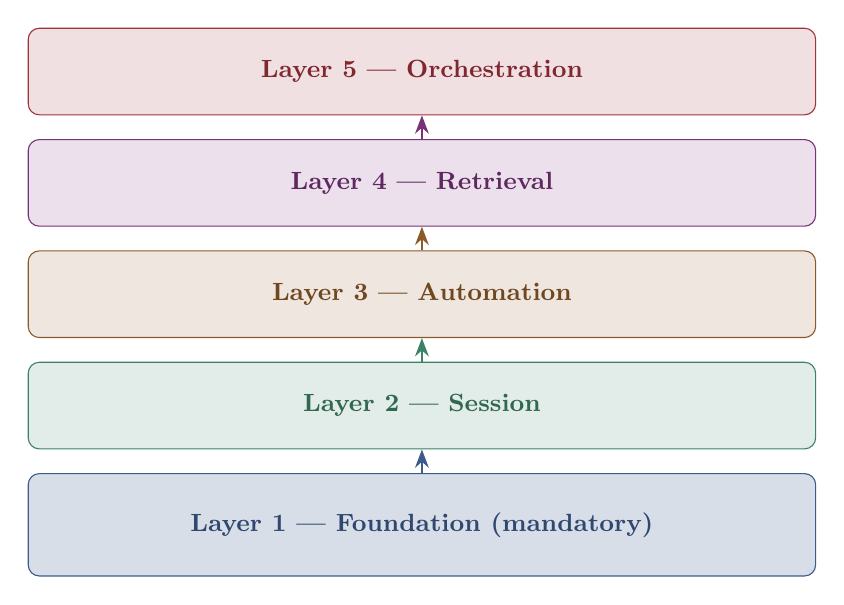
\begin{tikzpicture}[
  box/.style={rectangle, rounded corners=4pt, minimum width=10cm,
              minimum height=1.1cm, text centered, font=\small\bfseries,
              inner sep=8pt},
  arrow/.style={->, >=Stealth, thick}
]

\node[box, fill=l5color!15, draw=l5color, text=l5color!80!black]
  (l5) {Layer 5 --- Orchestration};
\node[box, fill=l4color!15, draw=l4color, text=l4color!80!black, below=0.3cm of l5]
  (l4) {Layer 4 --- Retrieval};
\node[box, fill=l3color!15, draw=l3color, text=l3color!80!black, below=0.3cm of l4]
  (l3) {Layer 3 --- Automation};
\node[box, fill=l2color!15, draw=l2color, text=l2color!80!black, below=0.3cm of l3]
  (l2) {Layer 2 --- Session};
\node[box, fill=l1color!20, draw=l1color, text=l1color!80!black, below=0.3cm of l2,
      minimum height=1.3cm]
  (l1) {Layer 1 --- Foundation (mandatory)};

\draw[arrow, color=l1color] (l1.north) -- (l2.south);
\draw[arrow, color=l2color] (l2.north) -- (l3.south);
\draw[arrow, color=l3color] (l3.north) -- (l4.south);
\draw[arrow, color=l4color] (l4.north) -- (l5.south);

\end{tikzpicture}
\end{center}

\subsection{What Each Layer Owns}

\begin{center}
\begin{tabular}{@{}p{3.5cm}p{2cm}p{7cm}@{}}
\toprule
\textbf{Responsibility} & \textbf{Layer} & \textbf{Mechanism} \\
\midrule
Permanent storage & 1 & Plain text files in folder hierarchy \\
Metadata & 1 & YAML frontmatter on standalone files \\
Version history & 1 & Versioned triplet files (v01, v02\ldots) and git \\
Project narrative & 1 & THREAD.md checkpoint log \\
Library navigation & 1 & MAP.md traversal index \\
Session control & 1 & Master prompt + commands \\
\midrule
Master prompt auto-loading & 2 & CLAUDE.md import (Claude Code) \\
File-based RESUME & 2 & Skill reads persona + THREAD + latest context/instructions from disk \\
Reduced startup friction & 2 & No copy-paste required where file access exists \\
\midrule
Checkpoint parsing and saving & 3 & checkpoint.py \\
Structural validation & 3 & pre-commit hook \\
Ritual orchestration & 3 & ai-library-ops skill \\
Note logging & 3 & add\_note\_thread.py \\
\midrule
Semantic search & 4 & Embedding model + vector store \\
Automatic context loading & 4 & search.py + load-context.py \\
Filtered retrieval & 4 & Frontmatter metadata + vector similarity \\
\midrule
Folder navigation by AI & 5 & MCP client reads library directly \\
Scheduled tasks & 5 & cron + API scripts \\
Cross-project synthesis & 5 & Synthesis agent reads all THREAD.md \\
Pipeline automation & 5 & run-pipeline.py orchestrates agents \\
Team collaboration & 5 & Shared folder + merge protocol \\
\bottomrule
\end{tabular}
\end{center}

\subsection{Implementation Sequence}

The recommended implementation sequence is strictly bottom-up.
Do not skip layers.

\begin{enumerate}
  \item \textbf{Layer 1:} Create the folder structure. Move existing
        files into \texttt{inbox/}. Sort one project. Create its
        \texttt{THREAD.md} and \texttt{persona.md}. Save
        \texttt{MASTER-PROMPT.md} to the library root. Run one
        complete session and call one checkpoint by hand. This is the
        proof of concept.

  \item \textbf{Layer 2:} Run several sessions from the project's
        natural environment (Claude Code, Cowork, or manual paste).
        Verify \texttt{RESUME} consistently reconstructs the right
        state from persona.md, THREAD.md, and the latest
        context/instructions files alone, with no missing context.

  \item \textbf{Layer 3:} Write or deploy the checkpoint script and
        pre-commit hook. Test on a real checkpoint output. Verify all
        four files save correctly and \texttt{THREAD.md}/\texttt{MAP.md}
        update accurately. Use it for ten real checkpoints before
        adding Layer 4.

  \item \textbf{Layer 4:} Choose an embedding model and vector store.
        Index the library. Run ten retrieval queries across different
        topics. Verify that results are accurate and relevant. Integrate
        retrieval into the session start workflow for one month.

  \item \textbf{Layer 5:} Implement MCP connection first, before any
        scheduling or pipelines. Run ten sessions via the MCP client.
        Then implement one scheduled task (the weekly synthesis is
        recommended as the first). Verify it produces useful output
        for one month before implementing pipelines.
\end{enumerate}

\subsection{Status of This Library}

\begin{center}
\begin{tabular}{@{}llp{6.5cm}@{}}
\toprule
\textbf{Layer} & \textbf{Status} & \textbf{Note} \\
\midrule
1 & Implemented & In daily use since project start; 30+ checkpoints \\
2 & Implemented & Multi-platform: Claude Code (CLI/cloud/iOS), Cowork \\
3 & Implemented & checkpoint.py, pre-commit hook, ai-library-ops skill \\
4 & Not implemented & Estimated 4--8 hours setup once undertaken \\
5 & Not implemented & Estimated 8--20 hours setup once undertaken \\
\bottomrule
\end{tabular}
\end{center}

% ---------------------------------------------------------------
\section{Document Index}

\begin{center}
\begin{tabular}{@{}lp{9cm}@{}}
\toprule
\textbf{File} & \textbf{Contents} \\
\midrule
\texttt{MASTER-PROMPT.md} &
The control mechanism for every AI session. Contains the complete
Layer 1 operating instructions for any AI model. \\
\texttt{CLAUDE.md} &
Imports \texttt{MASTER-PROMPT.md} so Claude Code sessions load it
automatically; the Layer 2 loading mechanism for this implementation. \\
\texttt{USER-GUIDE.tex} &
Practical, task-oriented guide: how to RESUME, CHECKPOINT, NOTE,
COMMIT, and start a NEW PROJECT, end to end. \\
\texttt{ARCHITECTURE.tex} &
This document. Complete five-layer architecture reference. \\
\bottomrule
\end{tabular}
\end{center}

% ---------------------------------------------------------------
\section*{Colophon}

\vspace{8pt}
\hrule height 0.4pt
\vspace{12pt}

\begin{center}
{\small\texttt{AI-Library / ARCHITECTURE.tex} \quad Version 2.0 \quad \today}\\[6pt]
{\small Plain text. Open format. No vendor. No application required. No expiry.}\\[4pt]
{\footnotesize
Layer 1 is the only mandatory layer.\\
Every additional layer adds convenience.\\
None of them changes where the truth lives.
}
\end{center}

\end{document}
